%TITLE, AUTHOR, DATE
\documentclass[12pt, a4paper]{article} %14 pt indicates the font size of the prepared document
\usepackage[margin=1in]{geometry}
\usepackage[utf8]{inputenc}
\usepackage{multicol}
\usepackage{multirow}
\usepackage{color}
\usepackage{enumerate}
\usepackage{amsmath}
\usepackage{graphicx}
\usepackage{calligra}
\usepackage{hyperref}
\usepackage{subcaption}



\title{CSE 300: Online Assignment}
\author{Md Shamsuzzoha Bayzid, Mahjabin Nahar, Md Shariful Islam Bhuyan,\\
	and Md Saidur Rahman
}
\date{June 2021}

\begin{document}
	\maketitle
	
	\section{Introduction}
	This assignment has been designed to assess the preparation of the students
	in writing scientific articles using \LaTeX. This assignment covers a variety of
	components that are commonly used in scientific manuscripts.
	

	
	\subsection{Equation}
	Let $a_0$, $a_n$ and $b_n$ are terms of a series. Their definitions are given by Eqn. 1.\\
	
	$
	a_0 = \frac{1}{\pi} \int_{-\pi}^{\pi}f(x)dx $ \\
	$a_1 = \frac{1}{\pi} \int_{-\pi}^{\pi} f(x)\cos nx dx = \frac{1}{\pi} \int_{-\pi}^{\pi} x^2\cos nx dx
	$ \\
	$
	a_1 = \frac{1}{\pi} \int_{-\pi}^{\pi} f(x)\sin nx dx = \frac{1}{\pi} \int_{-\pi}^{\pi} x^2\sin nx dx
	$
	\subsection{Tables}
	We wish to place the Table at the bottom of the page.
	
	\subsection{Figures}
	We intend to put Figure 1 at the top of a page.
	
	\pagebreak
%	
%		\begin{sidewaysfigure}[h]
%		\centering
%		\subfloat[First figure]{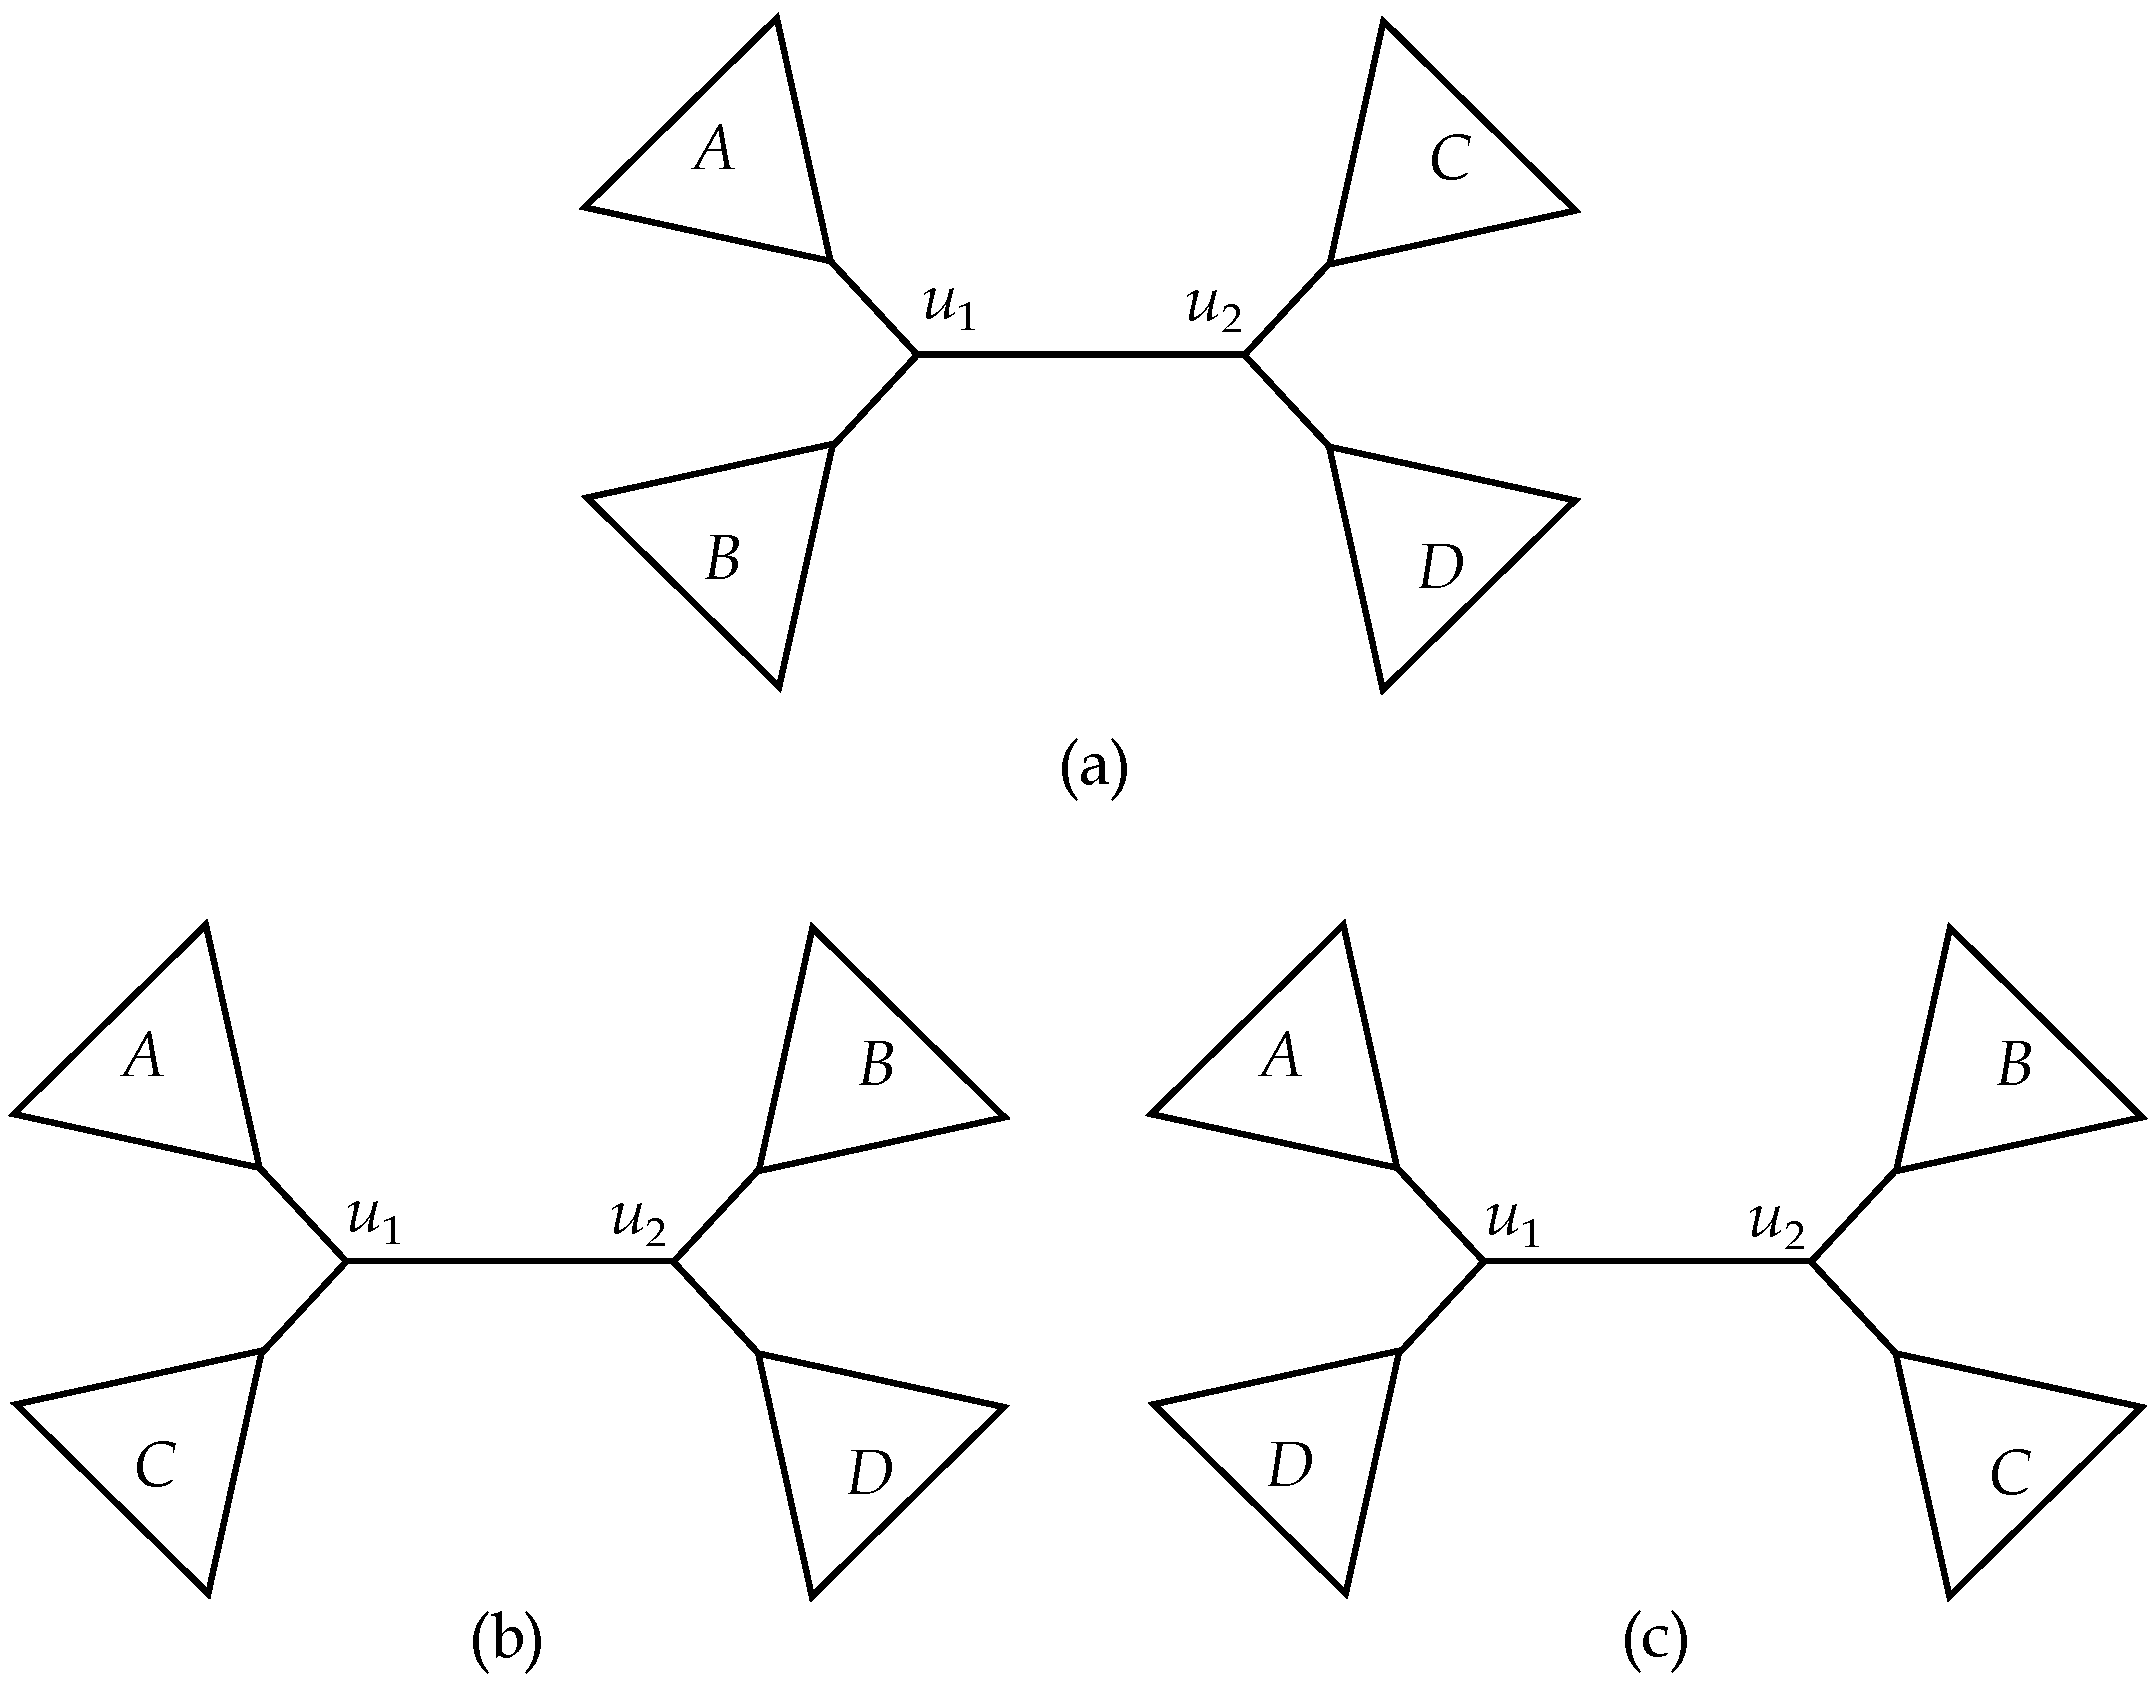
\includegraphics[width=0.28\textheight]{Figure.pdf}} \quad
%		\subfloat[Second figure]{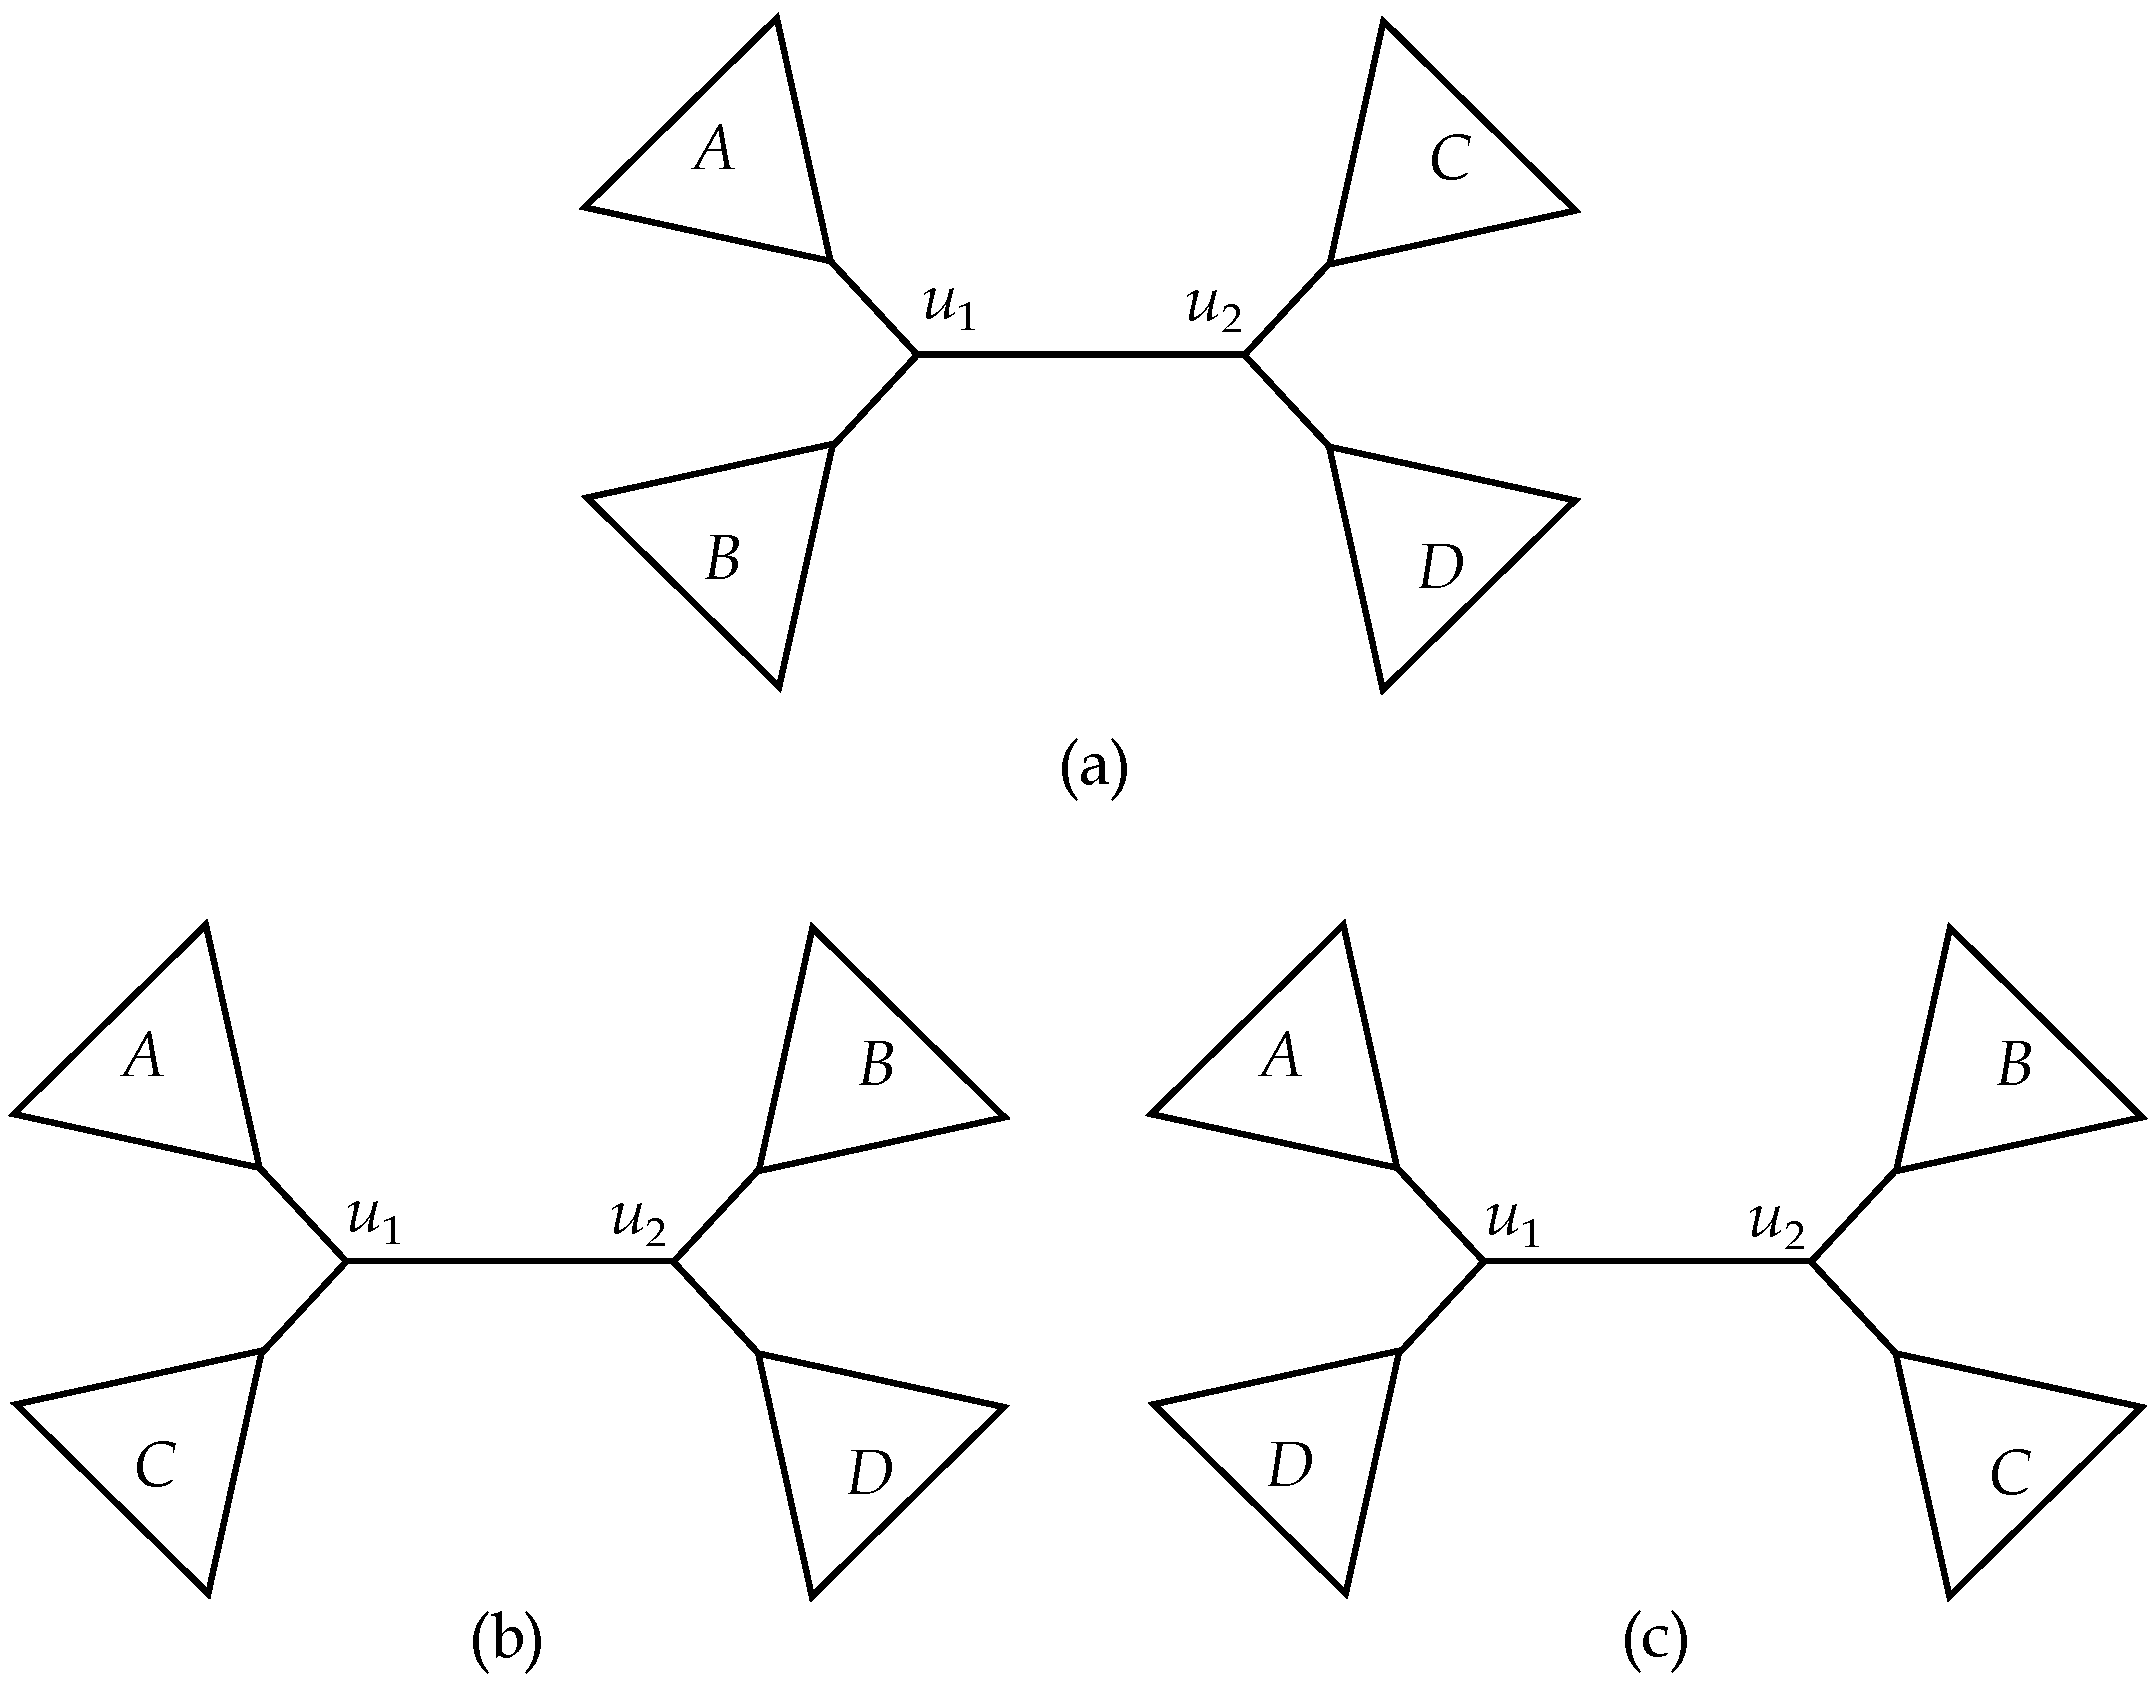
\includegraphics[width=0.28\textheight]{Figure.pdf}}\quad
%	\end{sidewaysfigure}
		
	\begin{figure}[h!]
		%...
		\centering
		\begin{subfigure}{0.5\textwidth}
			\centering
			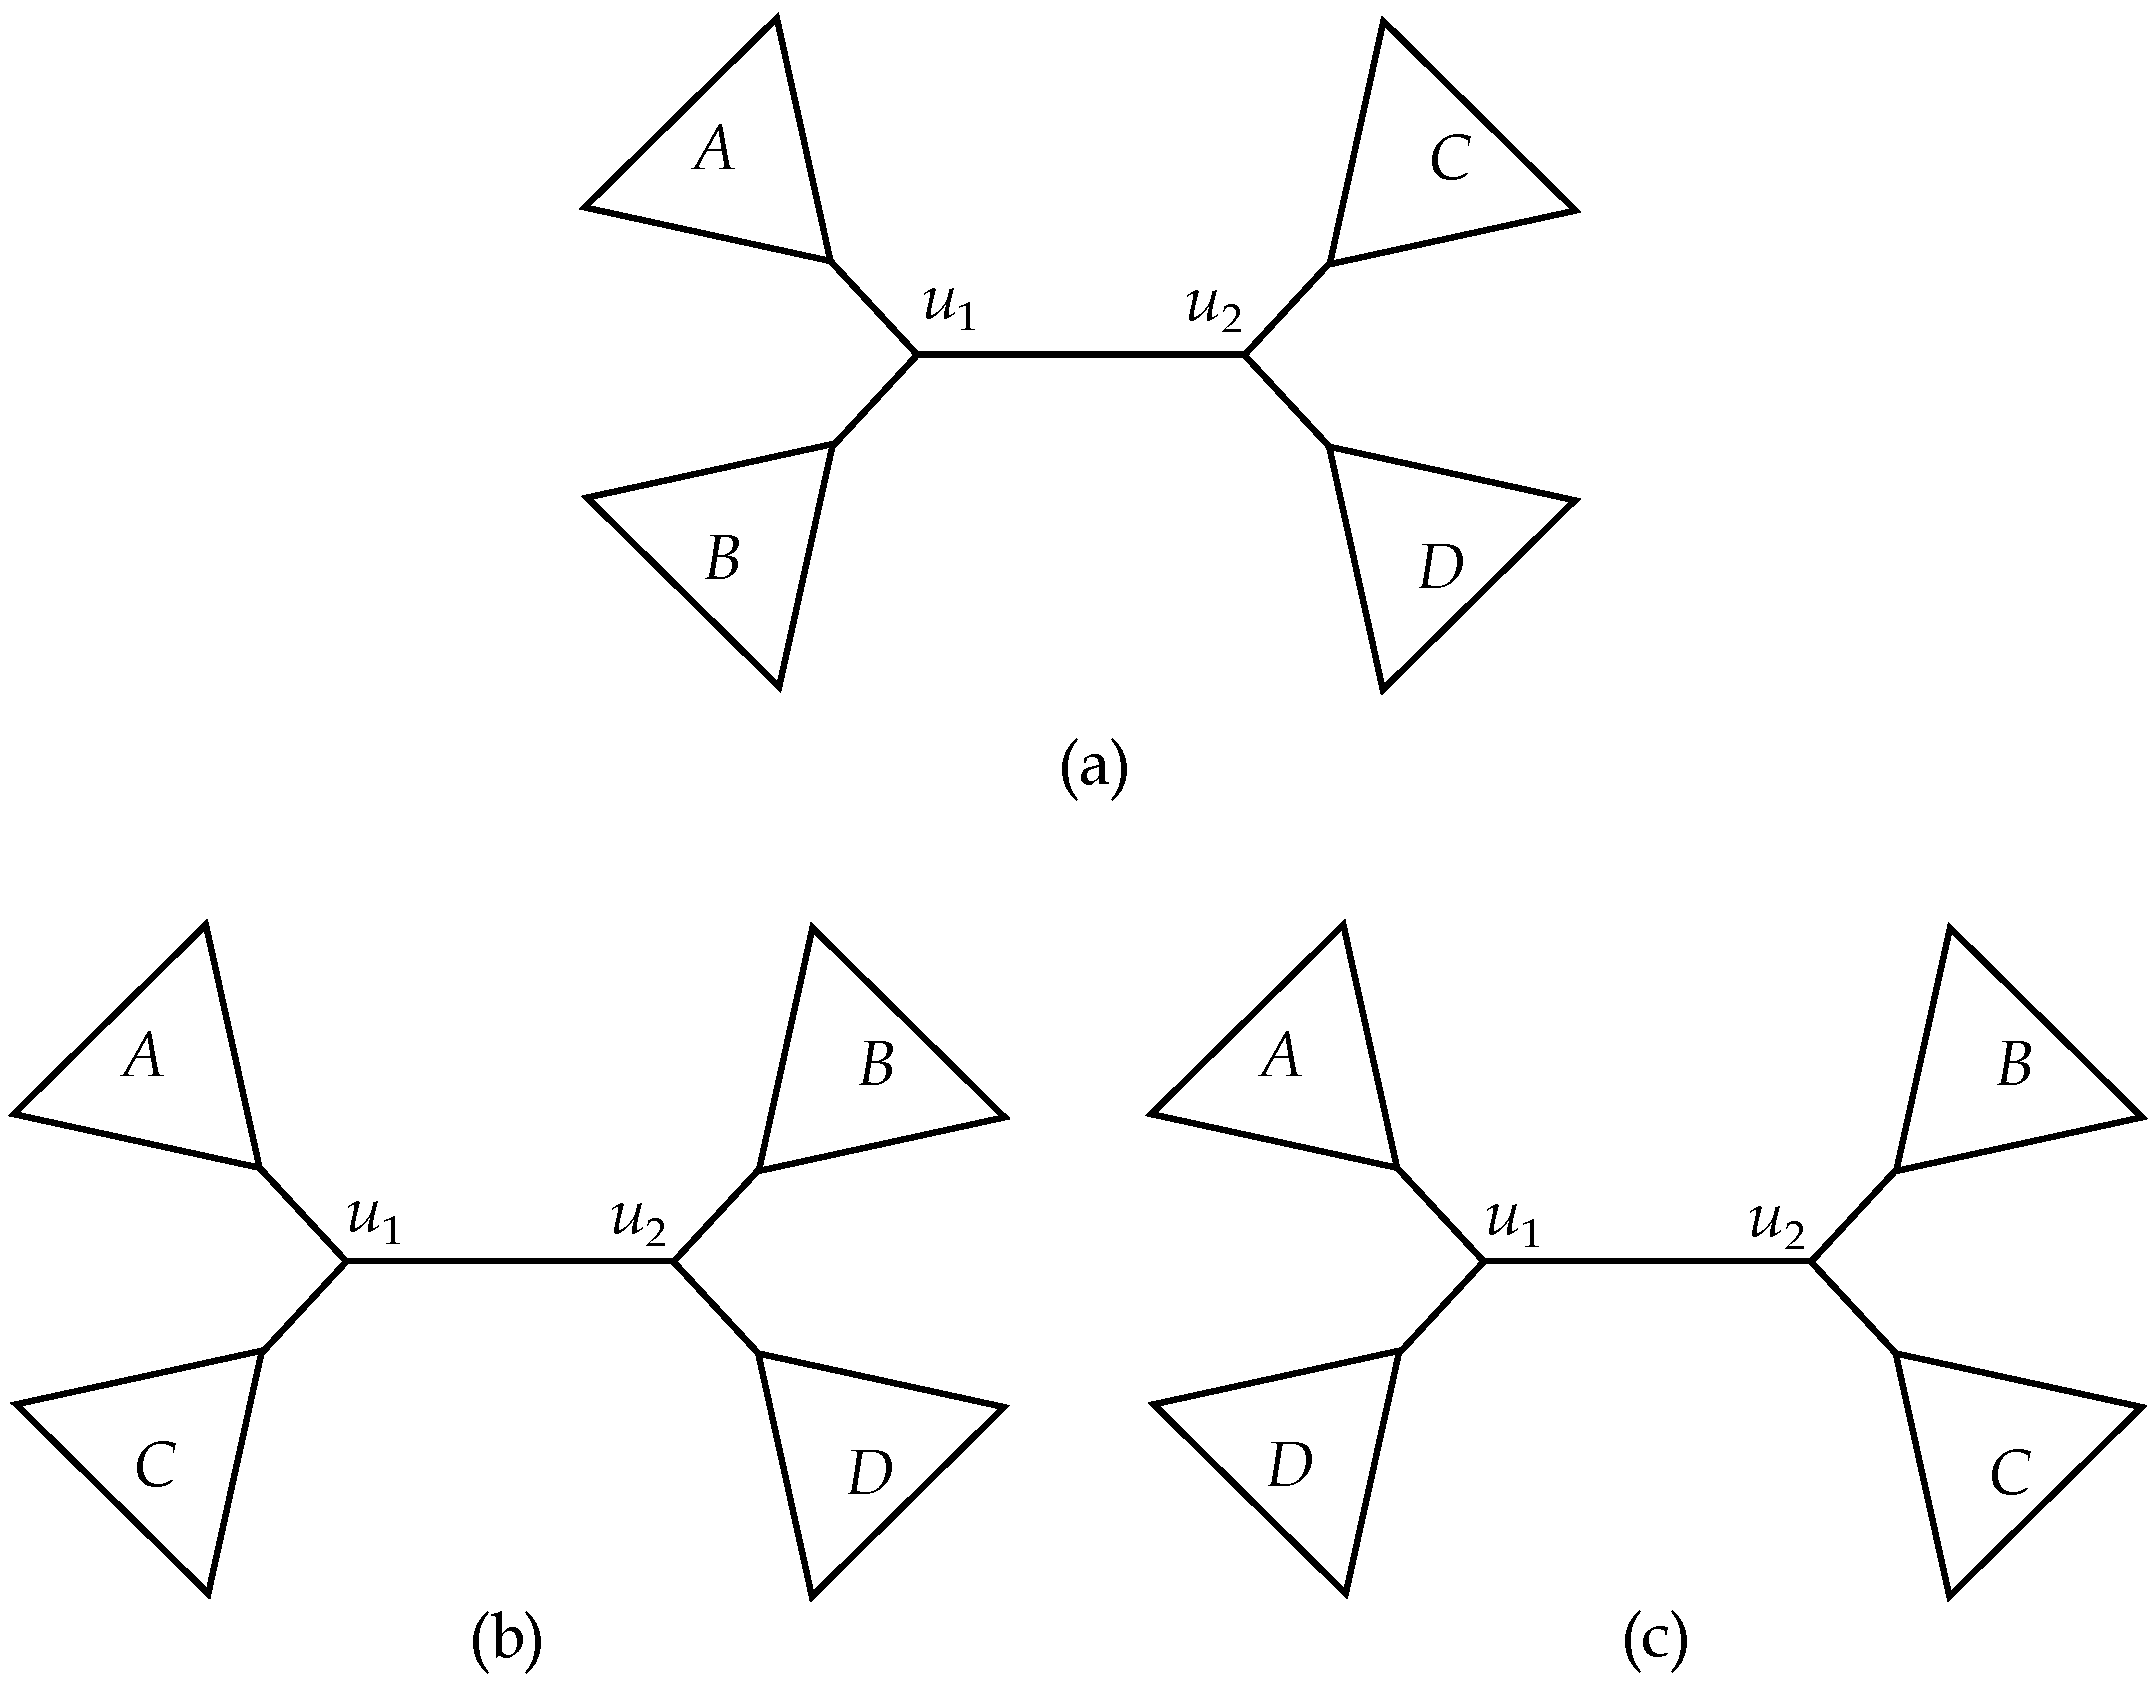
\includegraphics[width=.5\linewidth]{Figure.pdf}		
			
		\end{subfigure}%
		\begin{subfigure}{0.5\textwidth}
			\centering
			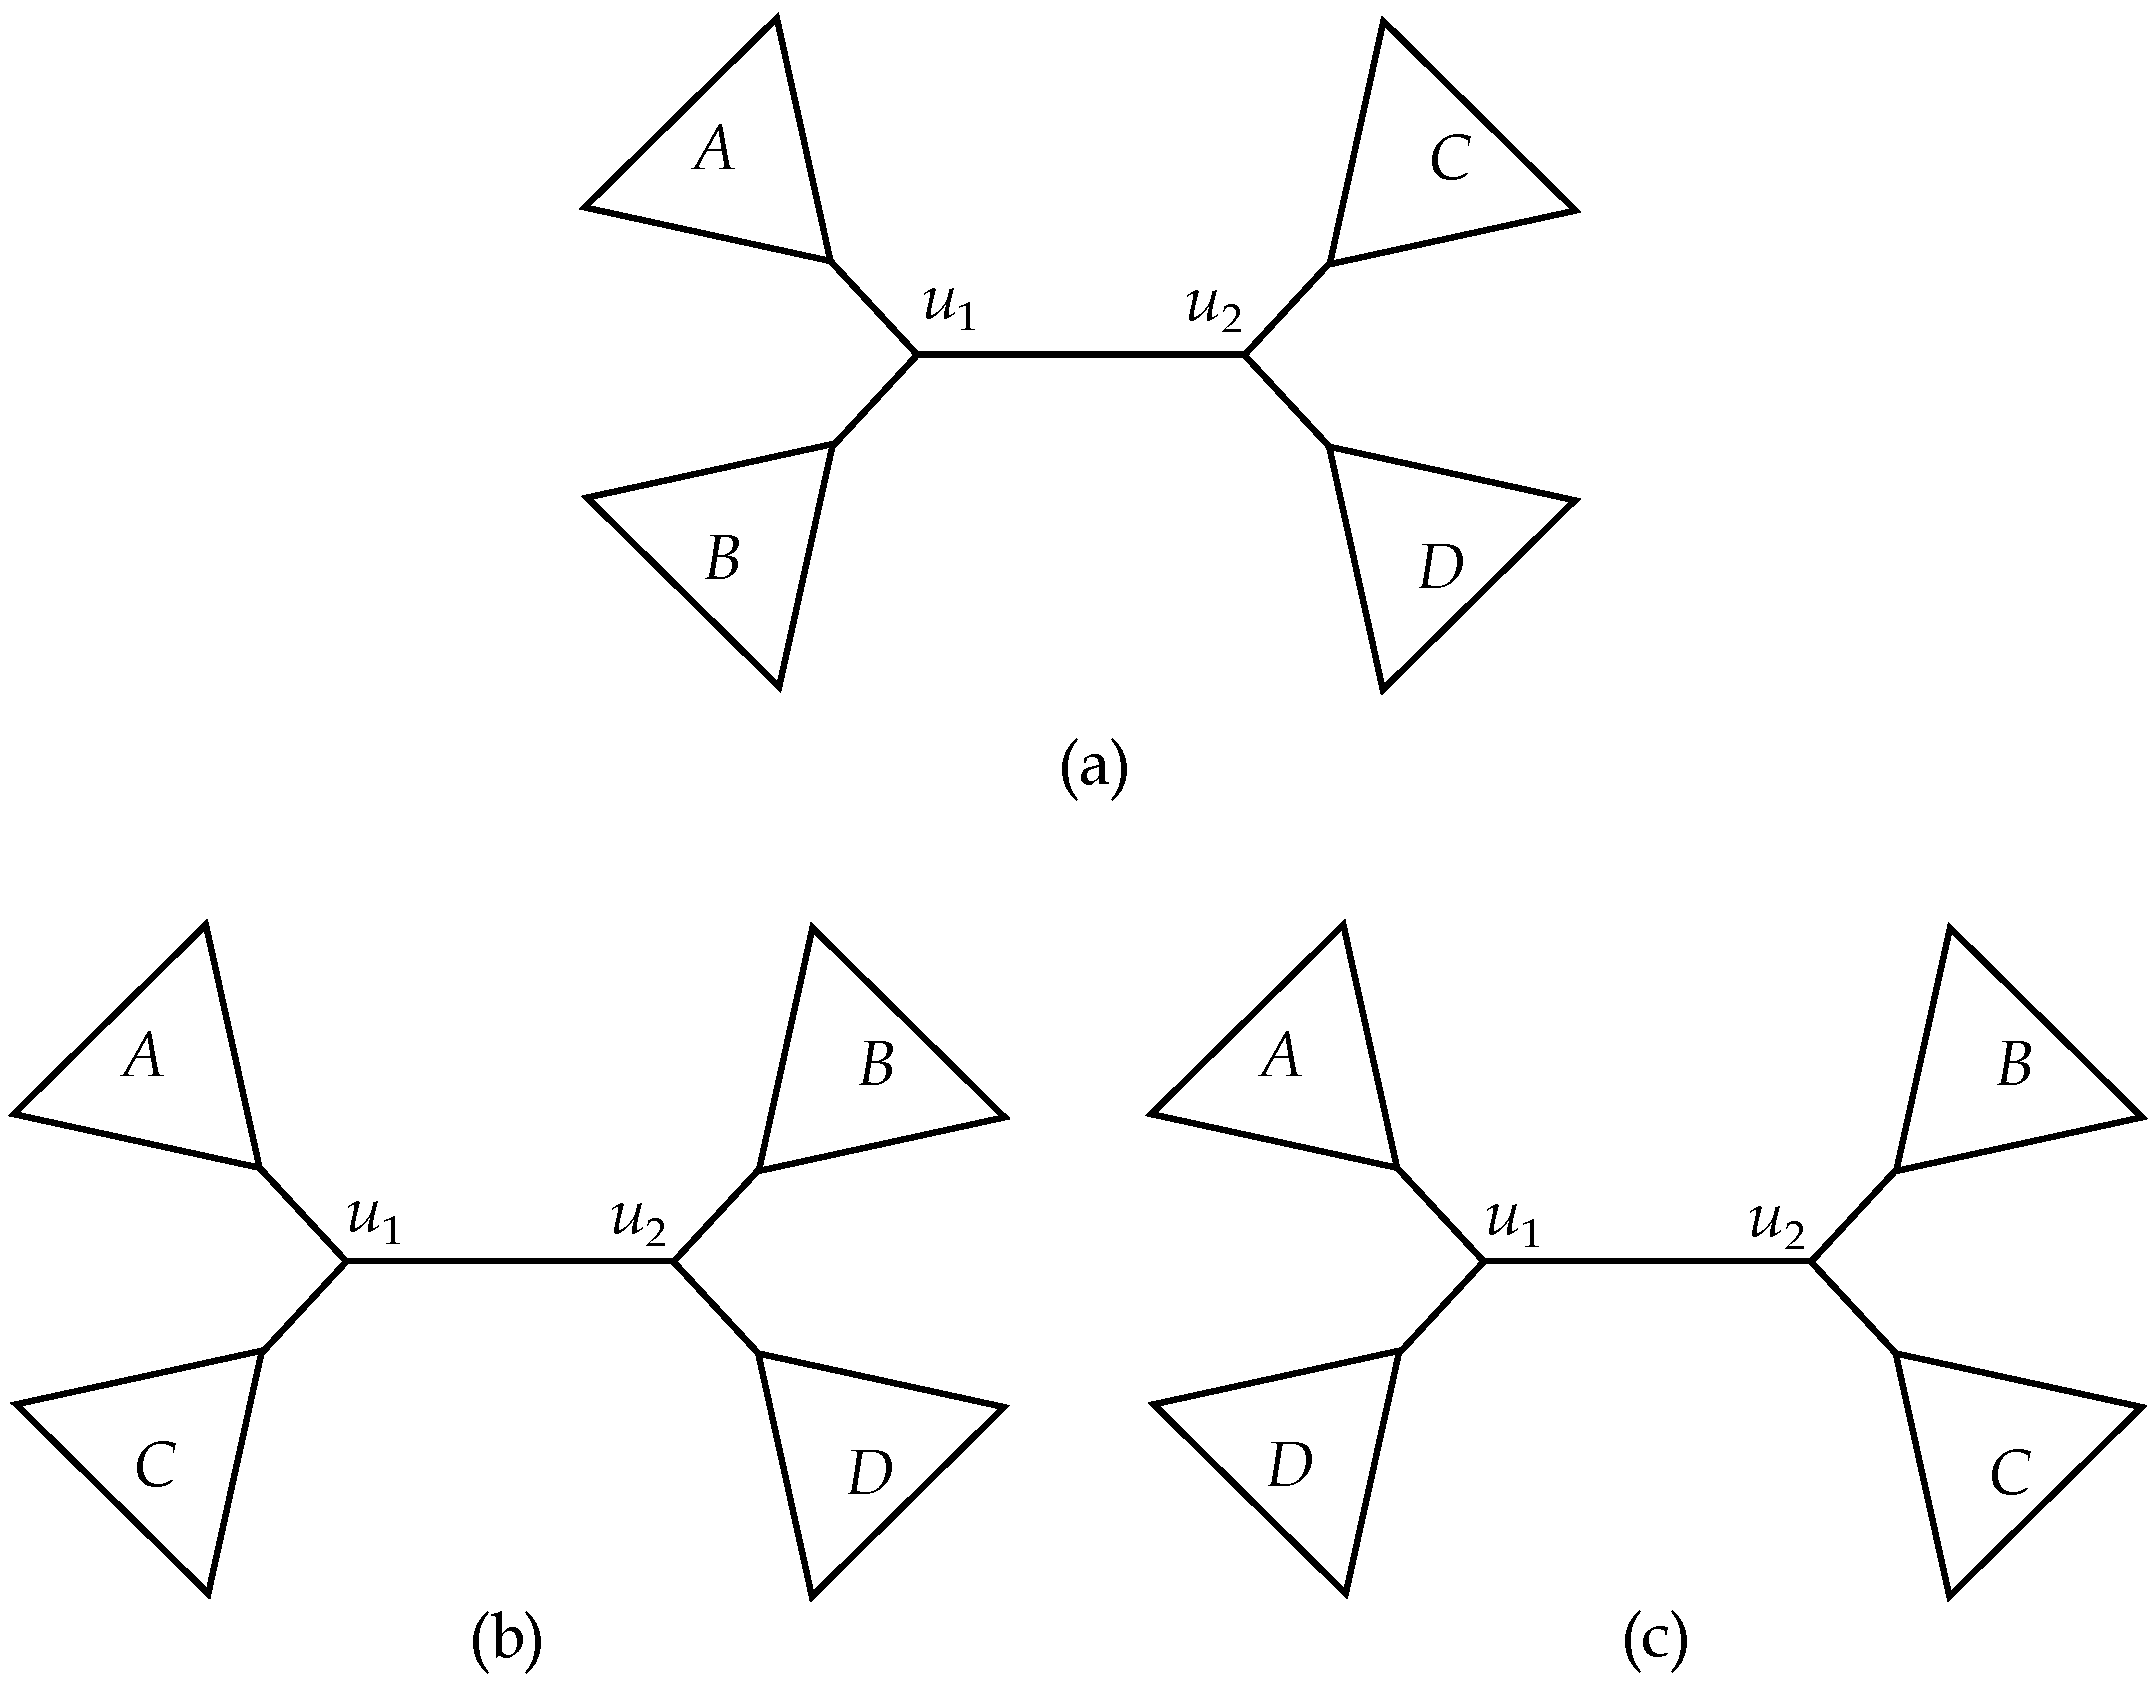
\includegraphics[width=.5\linewidth]{Figure.pdf}
		\end{subfigure}
		\caption{Side by side same figure}
	\end{figure}
	
	\section{Conclusions}
	The major objectives of this assignment are listed below (please do not ignore \\
	the font sizes).
	
	\begin{itemize}
		\Large{\item To assess the ability of the students in preparing
		manuscripts in \LaTeX.}
		\large{\item To see if the students have adequately practiced different
			aspects of writing in \LaTeX.}
	\end{itemize}
	
	\begin{table}[h]
		\centering
		
		\vspace{10mm}
		\begin{tabular}{|c||c|c|c|}
			\hline
			\multicolumn{4}{|c|}{Item List} \\  
			\hline
			Item Name or \newline Product name & ALPHA 2 Code & ALPHA 3 Code & Numeric Code \\
			\hline 
			Item001 & AF & AFG &
			\multirow{4}{*}{
			\begin{tabular}{|c|c|c|}
				004 & \multicolumn{2}{|c|}{}  \\ \cline{1-1}
				008 & \multicolumn{2}{|c|}{} \\ \cline{1-1}
				009 & \multicolumn{2}{|c|}{}  \\ \cline{1-3}
				012 & 013 & 014 \\ \hline
			\end{tabular}		
		}\\ 
				 
			Item002 & AX & ALA & \\ 
			Item003 & AL & ALB & \\
			Item004 & DZ & DZA & \\
			\hline \hline
			Item005 & AS & ASM & 
			\multirow{3}{*}{
			\begin{tabular}{|c|c|}
				016 & \\ \hline
				010 & 020 \\ \hline
				024 & 025 \\ \hline
			\end{tabular} 	
		} \\
			
		   Item006 & AD & AND & \\
		   Item007 & AO & AGO & \\ \hline \hline
			
			
			
		\end{tabular}
	\end{table}
	\newpage
	

	\begin{itemize}
		{  \item To see if the students can add various basic components (e.g., tables,
			figures, equations) to a \LaTeX  manuscript.}
		{\item To see if the students can leverage the available materials (both offline and
			online) to do something which has not explicitly been taught in the class.}		
	\end{itemize}	
	
\end{document}
